\section{Aufteilung des Trainingsdatensatzes}
\label{chap:Trainingssplit}
Nachdem die Attribute codiert wurden und der Datensatz somit in eine Form gebracht wurde, die zum Anlernen eines \ac{KI}-Modells geeignet ist, 
muss nun als Nächstes eine Aufteilung in Trainings- und Testdaten sowie in Eingabe- und Ausgabewerte erfolgen. Da die Bewertung einer Anwendungsregel
unabhängig von der Bewertung anderer Anwendungsregeln ist, darf das \ac{KI}-Modell nur mit den Bewertungen zu der spezifischen Anwendungsregel angelernt werden.
Wie Abbildung \ref*{fig:ARMenge} jedoch zeigt, wurden nur 38 Anwendungsregeln mehr als zehnmal bewertet, die allermeisten Anwendungsregeln wurden nur weniger als 
fünfmal bewertet. Das sorgt dafür, dass beim \ac{KI}-Modell mit Überanpassung gerechnet werden muss, da der Datensatz zu klein ist.
\begin{figure}[H]
    \centering
    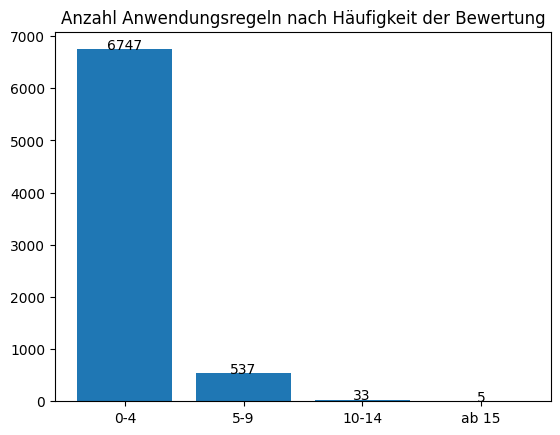
\includegraphics[width = \textwidth]{abbildungen/BalkenAR.png}
    \caption{Säulendiagramm zur Häufigkeit der Bewertung von Anwendungsregeln}
    \label{fig:ARMenge}
\end{figure}

Um den Datensatz auf die Bewertungen von Anwendungsregeln zu beschränken, welche gerade bewertet werden soll, wurde zur Demonstration dieses Schritts 
beispielhaft die Anwendungsregel ausgewählt, welche am häufigsten im Datensatz vorhanden war. Der Quellcode \ref*{lst:defTraining} zeigt den benötigten Code-Ausschnitt,
um diese Schritte durchzuführen.

\begin{lstlisting}[language = python, caption={Definieren des Trainingsdatensatzes},captionpos=b, label = lst:defTraining, floatplacement=H]
df_training = df
text = "Zur Anschaltung des Antriebes in der Außenanlage muessen Signalkabel nach VDE 0816/2 oder Kabel mit vergleichbaren Eigenschaften verwendet werden. Die Verlegevorschriften des Kabels sind einzuhalten."
df_training = df_training.loc[df_training['Text'] == text]

trainX = drop_columns(df_training, ['Status', 'Text', 'Statement'])
trainYStatus = drop_column(column_one_hot(df_training[['Text', 'Status']], ['Status']), "Text")
trainYStatement = drop_column(column_one_hot(df_training[['Text', 'Statement']], ['Statement']), "Text")
\end{lstlisting}

Zeile 2 des Quellcodes \ref*{lst:defTraining} speichert den beispielhaft ausgewählten Text einer Anwendungsregel in eine Variable. Bei der späteren Anwendung würde dieser Text
aus dem Modul in \ac{DOORS} extrahiert werden. In der nächsten Zeile wird der Datensatz auf die Zeilen beschränkt, die als Text den ausgewählten Text besitzen.
Die letzten drei Zeilen werden für die Aufteilung in Eingabe- und Ausgabewerte benötigt. Alle Spalten, bis auf die beiden Ausgabewerte \glqq Status\grqq{} und 
\glqq Statement\grqq{} sowie der Text der Anwendungsregel, stellen die Eingabewerte dar. Die beiden Ausgabewerte mussten in jeweils eigene Dataframes aufgeteilt werden, 
der Grund dafür wird in Kapitel XXX beschrieben.

Nun sind die Daten korrekt codiert und aufgeteilt in einen Trainingsdatensatz mit getrennten Ein- und Ausgabewerten. Der Testsplit wird beim Anlernen definiert, näheres dazu ebenfalls in Kapitel XXX.